\chapter{Pruebas de escala}
En esta sección se listarán las distintas pruebas de escala realizadas. Se explicará el propósito de cada prueba, las características de cada una de ellas (topologias, tipos de tráfico, etc) y por último, los resultados que arrojan.

\section{Funcionamiento básico para distintas topologias}
La idea de esta prueba es en cierta manera extender las pruebas que ya fueron realizadas por el proyecto RRAP, y corroborar el funcionamiento básico de la arquitectura y de la aplicación para topologias de diferentes tamaños y características.
\subsection{Descripción del escenario}
El objetivo es crear una VPN de capa 3 entre dos subredes CE, que permita tráfico de ethertype \textbf{0x0800}, es decir, tráfico del protocolo IPv4. Luego se generan datos y se envían por la VPN. De esta forma, se prueba que funcionan correctamente las siguientes funcionalidades.

\begin{itemize}
	\item Algoritmo de ruteo. Se verifican dos aspectos claves: que el camino se corresponde con el camino esperado (calculado previamente de forma manual), y que el camino es correctamente instalado en forma de reglas de reenvío (en base a conmutación de etiquetas MPLS) en las respectivas tablas de flujos OpenFlow de cada nodo del camino. Todo esto se puede comprobar analizando las tablas de flujos de cada nodo, que se pueden ver utilizando el comando \textbf{dump-flows} de OpenVSwitch. También se puede utilizar la interfaz gráfica de RAUFlow. Desde las tablas de flujos se puede reconstruir el camino que computó la aplicación, y también comprobar que los flujos configuran correctamente las etiquetas MPLS.
	
	\item Clasificación de tráfico. La idea es verificar que realmente se están asignando las etiquetas MPLS al tráfico entrante, así como comprobar que el mismo es reenviado por los nodos correctos. Para ello se genera tráfico utilizando el comando \textbf{ping} y la herramienta \textbf{iperf}. Con la herramienta tcpdump, se verifica el tráfico que pasa por cada nodo del camino.
\end{itemize}

Para comprobar que el comportamiento es consistente, las pruebas son realizadas con las siguientes topologias:
\begin{itemize}
	\item Básica: 4 RAUSwitch, en topología de full mesh. Es la utilizada en el prototipo físico.
	\item Chica: topología arbitraria de 11 nodos (fuente: Topology Zoo). Figura \ref{fig:topo_chica}.
	\item Mediana: topología arbitraria de 45 nodos (fuente: Topology Zoo). Figura \ref{fig:topo_mediana}.
	\item Grande: topología arborescente de 100 nodos
\end{itemize}

\begin{figure}[t]
\caption{Topología chica}
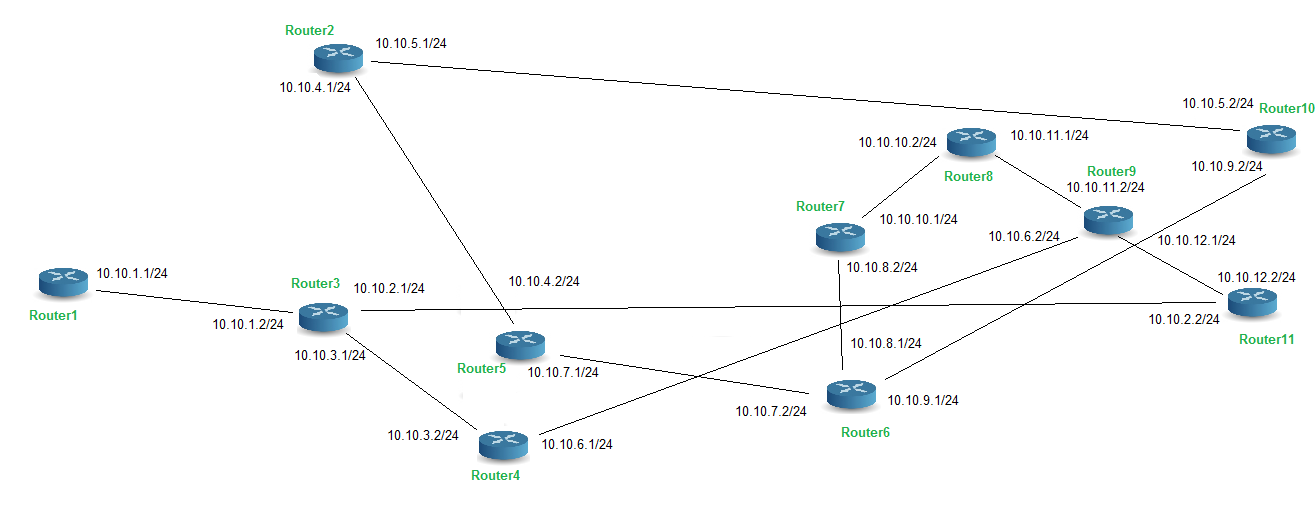
\includegraphics[scale=0.4]{Pruebas/topo_chica}
\centering
\label{fig:topo_chica}
\end{figure}

\begin{figure}[t]
\caption{Topología mediana}
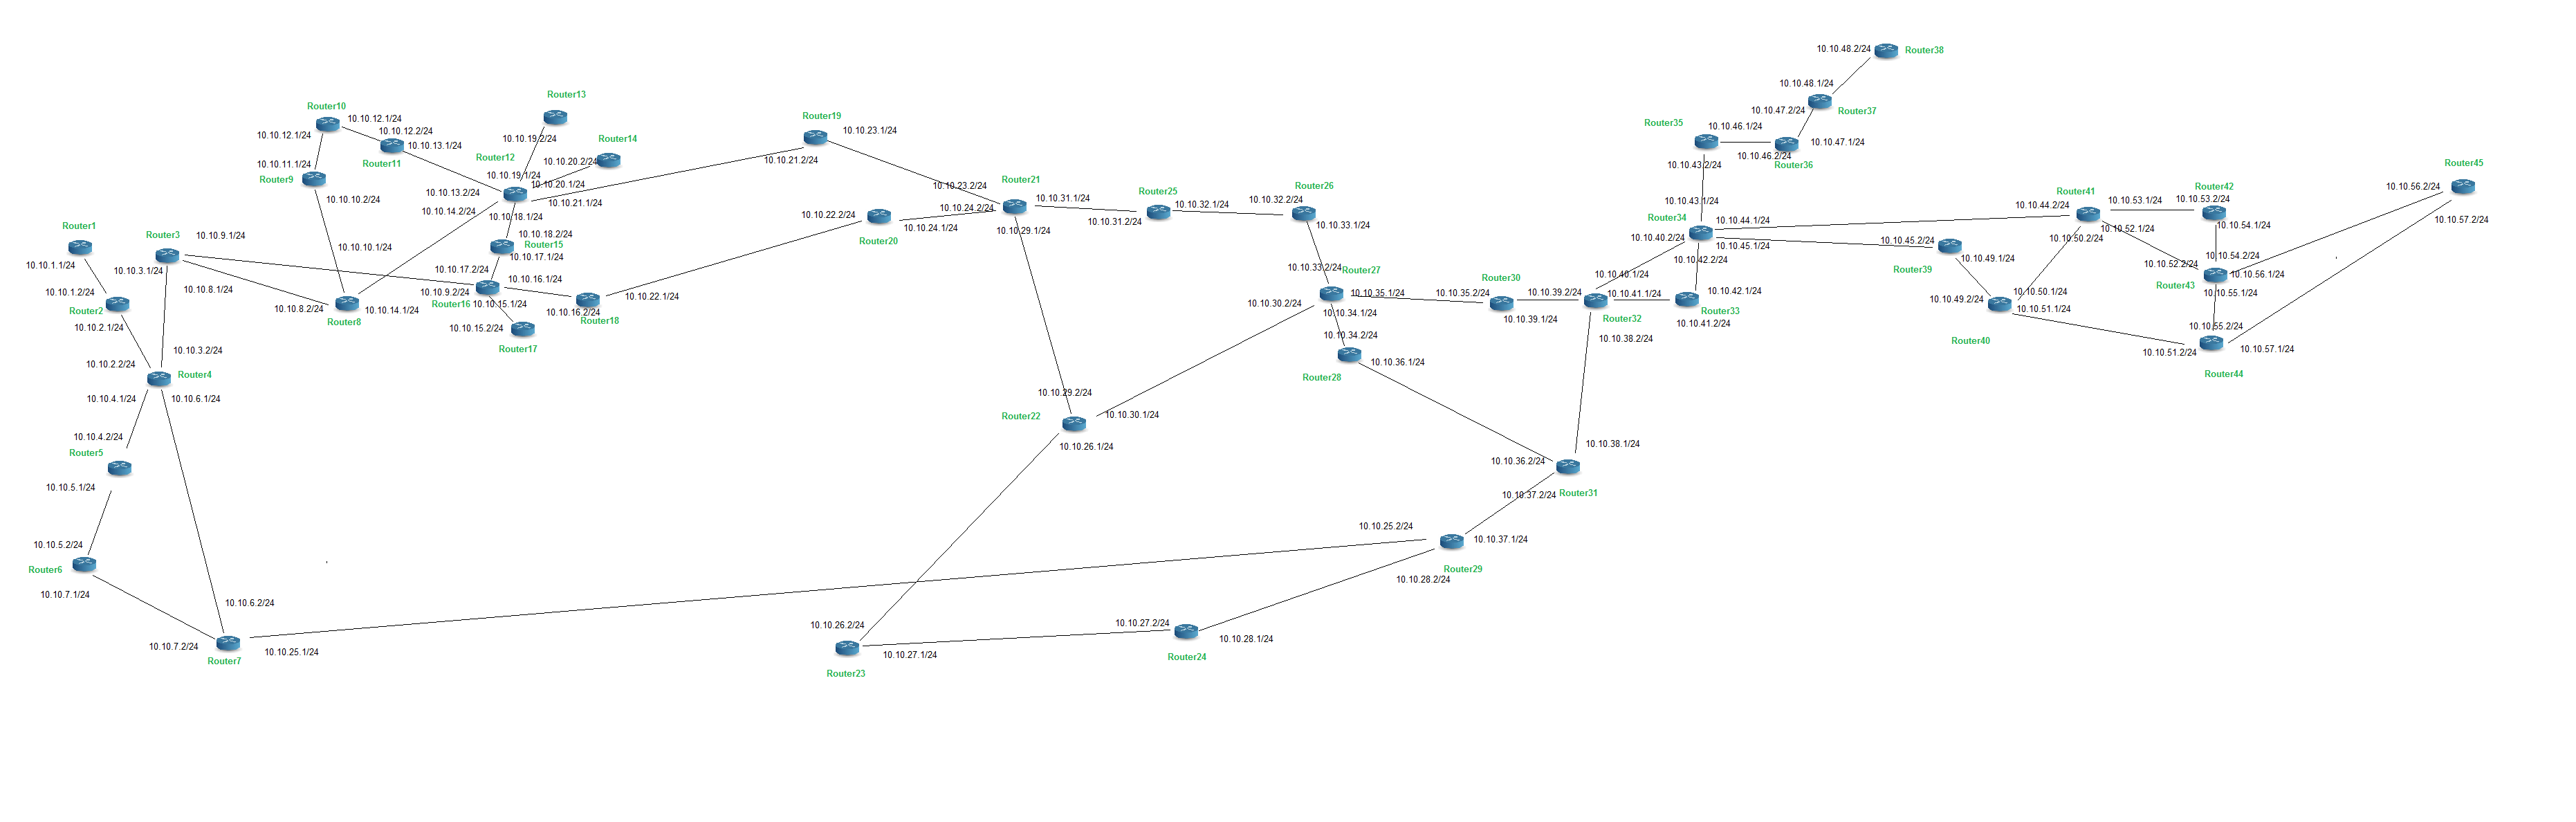
\includegraphics[scale=0.15]{Pruebas/topo_mediana}
\centering
\label{fig:topo_mediana}
\end{figure}

\subsection{Resultados y observaciones}
\textbf{Problema del MTU al usar iperf} \\
Hay que reducir 5 o 10 bytes (dependiendo de si el servicio usa 1 o 2 niveles de etiquetas MPLS) al MTU para que el tráfico pase.\\
\textbf{Bug en codigo (ruta)} \\
Error en el código que hacía que se instalaran mal los flujos en los nodos. Tenian incorrectos puertos de entrada y salida.\\
\textbf{Bug en codigo (Dijkstra)} \\
Error en el código del algoritmo de Dijkstra que hacia que se calcularan mal los costos, ya que se sumaba como strings (concatenación) en vez de sumar enteros.

\section{Escala de servicios y flujos}
Es probable que si un arquitectura de este estilo fuera desplegada en la Red Académica Uruguaya, sería sujeta a grandes cantidades de tráfico y, en particular, grandes cantidades de servicios. Por eso es de gran interés realizar pruebas sobre la misma que analicen su comportamiento cuando debe manejar decenas de miles, o incluso millones de flujos distintos. De esta forma se podrían identificar posibles puntos de falla, o umbrales bajo los cuales debe mantenerse la red para funcionar con buen rendimiento.

\subsection{Descripción del escenario}
Para estas pruebas se utiliza una topología básica de 4 RAUSwitch y dos subredes, como indica la figura \ref{fig:stress_servicios_topologia}. Se crean 15.000 VPNs de capa 2 entre las subredes, variando los cabezales OpenFlow para que toda VPN sea distinta de las demás. Además, se crea una VPN de capa 3 entre los mismos nodos, para permitir pasar el tráfico IP entre los hosts, que es el que se utiliza en las pruebas.

\begin{figure}[t]
	\caption{Topología para prueba de escala de servicios.}
	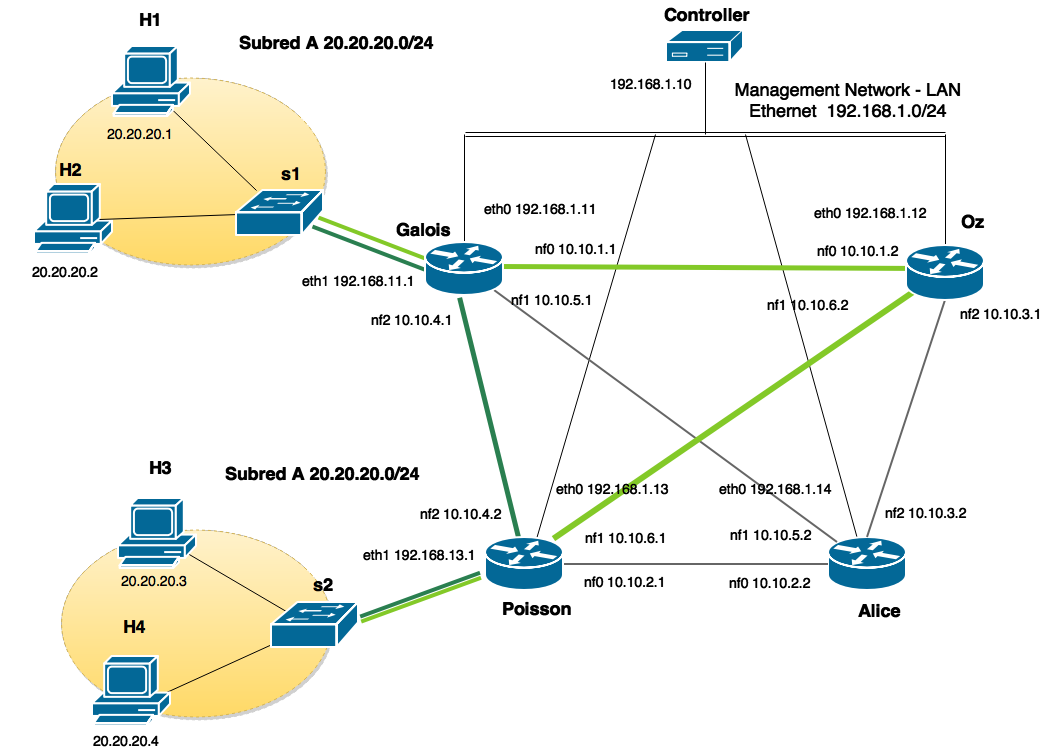
\includegraphics[scale=0.15]{Pruebas/stress_servicios_topologia}
	\centering
	\label{fig:stress_servicios_topologia}
\end{figure}

Interesa realizar estas pruebas estudiando dos aspectos claves:
\begin{itemize}
	\item Escalabilidad interna del RAUSwitch. Se estudian posibles limitaciones internas que puedan tener los dispositivos, cuando deben manejar grandes cantidades de flujos.
	\item Escalabilidad en servicios. Se estudian posibles problemas que puedan tener la arquitectura de la red o la aplicación del controlador para manejar grandes cantidades de servicios e información.
\end{itemize}


\subsection{Resultados y observaciones}
El comportamiento de la arquitectura al manejar esa cantidad de servicios es consistente, por lo tanto, es posible afirmar que la arquitectura de la red no tiene limitaciones con respecto a la cantidad de servicios. Sin ser una limitación, pero sí un factor importante, hay que recordar que los datos que maneja el controlador (entre ellos, los servicios) están en memoria. Por lo tanto se podrá agregar servicios mientras la computadora subyacente tenga suficiente memoria. La creación de 15.000 servicios aumenta el consumo de memoria del controlador en 205 Mb (CONFIRMAR), por lo que un servicio ocupa alrededor de 14 Kb. A modo de ejemplo, si extrapolamos ese número a una computadora que puede dedicar 4 Gb de RAM al controlador, llegamos a que dicho controlador podrá mantener alrededor de 300.000 servicios.


El otro aspecto de interés, la escalabilidad interna del RAUSwitch, arroja resultados similares. En teoría, cuantos más flujos en la tabla, más debería demorar el switch OpenFlow en encontrar el flujo que corresponde con el tráfico que está analizando, y por lo tanto el paquete demora más en ser forwardeado. Esto debería tener un impacto directo en el throughput. Como ya fue explicado, para comprobar esto se crearon 15.000 VPNs de capa 2. Esto implica alrededor de 1.260.000 flujos en ambos nodos, ya que cada VPN consiste de 2 servicios, y cada servicio de capa 2 instala 42 flujos en los nodos involucrados. Con la herramienta 'iperf', se crea tráfico TCP entre hosts de distintas subredes y se mide el throughput promedio sin las VPNs y con ellas. Ambos números resultan iguales, lo cual implica que la velocidad de transferencia no es afectada por más de un millón de flujos.\\
La explicación de este resultado se encuentra en la especificación de la herramienta OpenvSwitch, que utiliza la arquitectura para implementar OpenFlow. Dicha herramienta realiza cacheo de flujos, es decir, cuando el paquete de un determinado flujo llega por primera vez a un nodo, este paquete es enviado al pipeline de OpenFlow para determinar que acción se debe tomar. Luego de realizada, esta acción es escrita en la caché, y tiene un tiempo de vida de entre 5 y 10 segundos. Si en ese período de tiempo llega otro paquete del mismo flujo, no hay necesidad de enviar el paquete al pipeline, porque que ya se sabe cuales son las acciones a tomar para ese paquete. Por lo tanto, si un flujo de datos es constante y rápido, no importa cuántos flujos OpenFlow tenga el nodo, ya que sólo el primer paquete de ese flujo deberá pasar por el pipeline, y por ende, solo él se verá demorado por la existencia de muchos flujos.
\\

Mediante el comando 'ovs-appctl dpctl/show' de OpenVSwitch, podemos examinar las estadísticas del datapath para cada instancia de OpenVSwitch de nuestro entorno. En las figuras \ref{fig:iperf_sample} y \ref{fig:cache_sample} se observa, por un lado, la salida de 'iperf' luego de hacer tres ejecuciones, y por otro, las estadísticas del nodo 'alice' luego de dichas ejecuciones. En la sección 'lookups' se detallan cuantos 'hits' y 'miss' de caché han ocurrido hasta el momento, y 'flows' indica cuantos flujos activos hay en el momento en la caché.
\begin{figure}[t]
	\caption{Estadísticas de cache de flujos del nodo 'alice'.}
	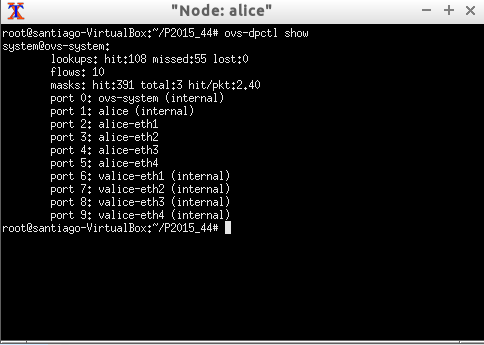
\includegraphics[scale=1]{Pruebas/cache_sample}
	\centering
	\label{fig:cache_sample}
\end{figure}

\begin{figure}[t]
	\caption{Resultado de la ejecución de 3 pruebas iperf en el host h1.}
	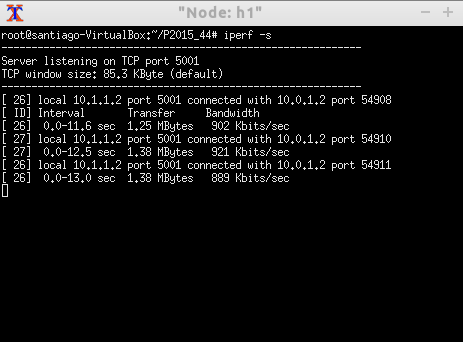
\includegraphics[scale=1]{Pruebas/iperf_sample}
	\centering
	\label{fig:iperf_sample}
\end{figure}